\begin{figure}[H]
\centering
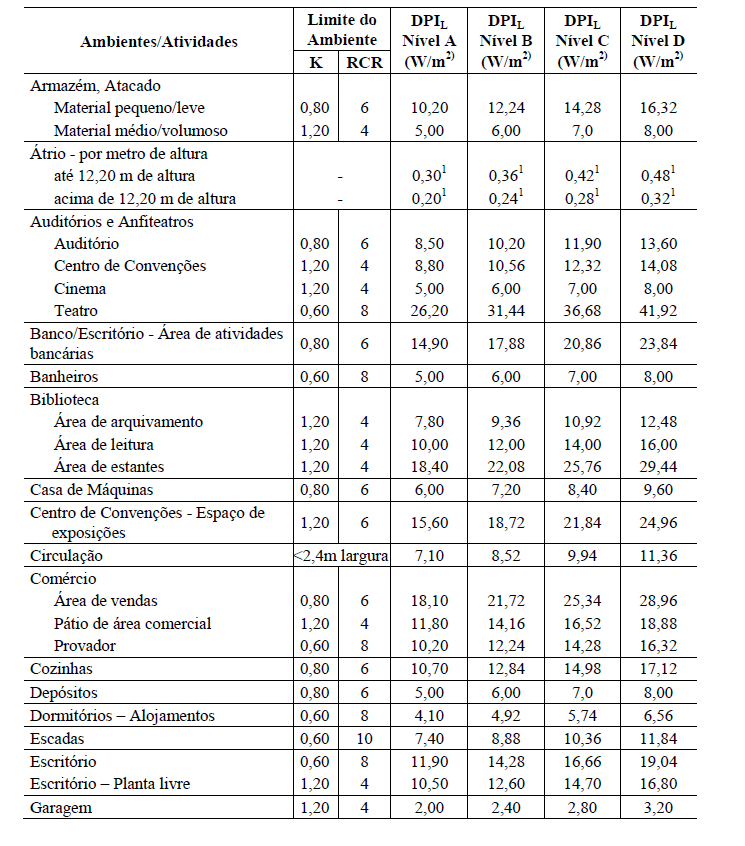
\includegraphics[width = 1.1\textwidth]{Figuras/tab1_1.PNG}
\caption{Limite máximo aceitável de densidade de potência de iluminação ($DPI_L$) para o nível de eficiência pretendido – Método das atividades do edifício.}
\label{tab2_1}
\textbf{Fonte:} Retirado de \cite{RTQ-C}.
\end{figure}

\begin{figure}[H]
\centering
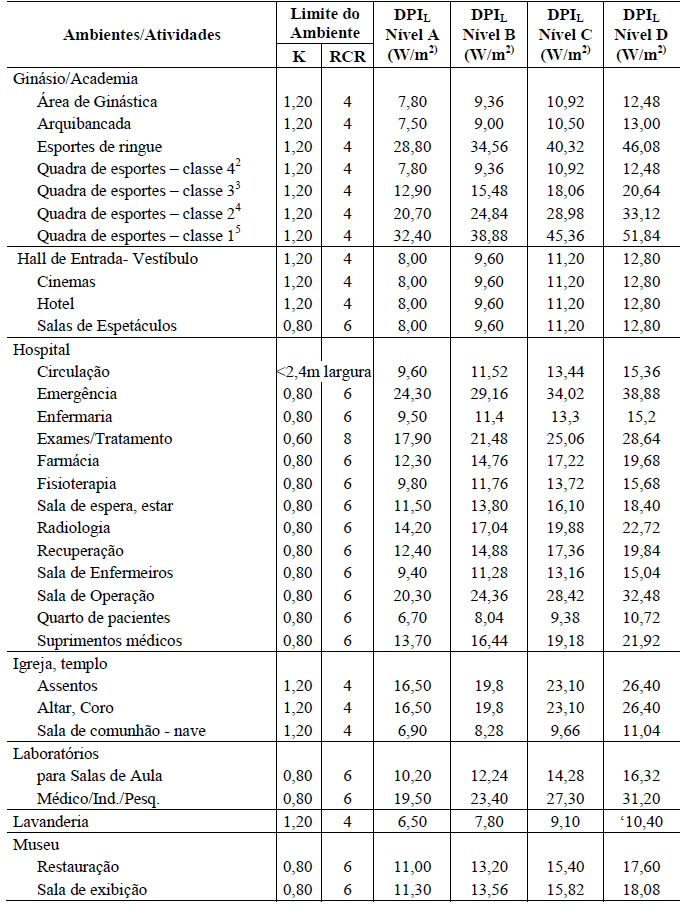
\includegraphics[width = 1.1\textwidth]{Figuras/tab1_2.PNG}
\caption{Limite máximo aceitável de densidade de potência de iluminação ($DPI_L$) para o nível de eficiência pretendido – Método das atividades do edifício(continuação).}
\label{tab2_2}
\textbf{Fonte:} Retirado de \cite{RTQ-C}.
\end{figure}

\begin{figure}[H]
\centering
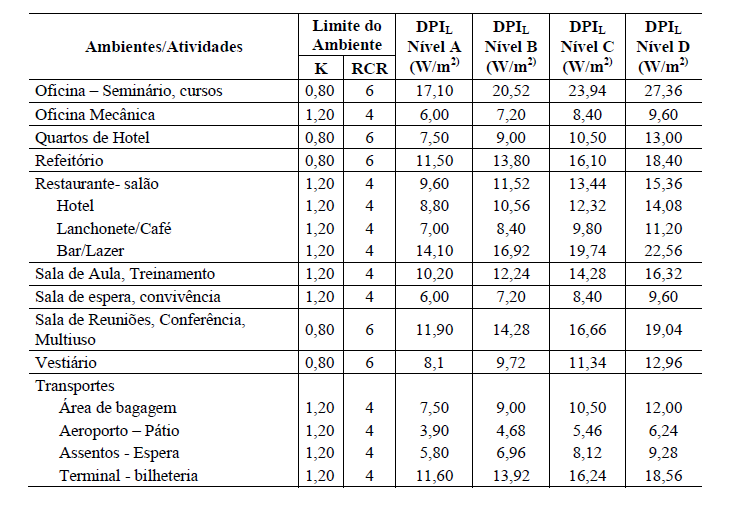
\includegraphics[width = 1.1\textwidth]{Figuras/tab1_3.PNG}
\caption{Limite máximo aceitável de densidade de potência de iluminação ($DPI_L$) para o nível de eficiência pretendido – Método das atividades do edifício(continuação).}
\label{tab2_3}
\textbf{Fonte:} Retirado de \cite{RTQ-C}.
\end{figure}